\documentclass[]{article}
\usepackage{lmodern}
\usepackage{amssymb,amsmath}
\usepackage{ifxetex,ifluatex}
\usepackage{fixltx2e} % provides \textsubscript
\ifnum 0\ifxetex 1\fi\ifluatex 1\fi=0 % if pdftex
  \usepackage[T1]{fontenc}
  \usepackage[utf8]{inputenc}
\else % if luatex or xelatex
  \ifxetex
    \usepackage{mathspec}
    \usepackage{xltxtra,xunicode}
  \else
    \usepackage{fontspec}
  \fi
  \defaultfontfeatures{Mapping=tex-text,Scale=MatchLowercase}
  \newcommand{\euro}{€}
\fi
% use upquote if available, for straight quotes in verbatim environments
\IfFileExists{upquote.sty}{\usepackage{upquote}}{}
% use microtype if available
\IfFileExists{microtype.sty}{%
\usepackage{microtype}
\UseMicrotypeSet[protrusion]{basicmath} % disable protrusion for tt fonts
}{}
\usepackage[margin=1in]{geometry}
\ifxetex
  \usepackage[setpagesize=false, % page size defined by xetex
              unicode=false, % unicode breaks when used with xetex
              xetex]{hyperref}
\else
  \usepackage[unicode=true]{hyperref}
\fi
\hypersetup{breaklinks=true,
            bookmarks=true,
            pdfauthor={Ciencia de Datos},
            pdftitle={ITAM Análisis clickstream},
            colorlinks=true,
            citecolor=blue,
            urlcolor=blue,
            linkcolor=magenta,
            pdfborder={0 0 0}}
\urlstyle{same}  % don't use monospace font for urls
\setlength{\parindent}{0pt}
\setlength{\parskip}{6pt plus 2pt minus 1pt}
\setlength{\emergencystretch}{3em}  % prevent overfull lines
\setcounter{secnumdepth}{0}

%%% Use protect on footnotes to avoid problems with footnotes in titles
\let\rmarkdownfootnote\footnote%
\def\footnote{\protect\rmarkdownfootnote}

%%% Change title format to be more compact
\usepackage{titling}

% Create subtitle command for use in maketitle
\newcommand{\subtitle}[1]{
  \posttitle{
    \begin{center}\large#1\end{center}
    }
}

\setlength{\droptitle}{-2em}
  \title{ITAM Análisis clickstream}
  \pretitle{\vspace{\droptitle}\centering\huge}
  \posttitle{\par}
  \author{Ciencia de Datos}
  \preauthor{\centering\large\emph}
  \postauthor{\par}
  \predate{\centering\large\emph}
  \postdate{\par}
  \date{4 de noviembre de 2015}

\usepackage{graphicx}


\begin{document}

\maketitle


En un sitio Web, el análisis de \emph{``clicksstream''} es el proceso de
recolección, análisis y presentación de datos agregados sobre cada paso
que siguen los visitantes en una página web y en qué orden, es decir,
son el resultado de la sucesión de clicks del ratón por cada visitante.
Regularmente, dicho flujo o registro de información es almacenado en un
principio para la gestión de los registros y posteriormente son
analizados para producir estadísticas que resulten de utilidad.

\section{0. El problema por resolver}\label{el-problema-por-resolver}

Para realizar dicho análisis es necesario obtener y estudiar los datos
provenientes de los \emph{access.logs} principalmente porque son datos
no estructurados. Una vez estructurados, se necesitan quitar los
registros duplicados, sesionizar los datos y enriquecer los registros ya
que debido a las características que aporta cada registro, suelen no ser
suficientes para tener un análisis más detallado.

Cabe destacar que no sólo la resolución del problema llega hasta esta
fase, sino hasta la creación de un dashboard o tablero de estadísticas
que ayudan a visualizar las principales características de los datos;
por ejemplo, los usuarios que tienen más visitas, su tiempo de
permanencia, las páginas más visitadas, entre otras.

\section{1. Orquestación}\label{orquestacion}

Al igual que en el análsis de Text Miner, se optó por utilizar el
orquestador \href{http://luigi.readthedocs.org/en/stable/}{luigi}, pero
para el análisis de \emph{clickstream}, las ventajas que se utilizan son
las de \emph{modularidad}, \emph{robustez} e \emph{idempotencia}. Cabe
resaltar que para esta fase del proyecto, debido a que no se tienen
archivos access.log provenientes de \emph{D-space}, los archivos logs
fueron obtenidos de diversas fuentes que serán mencionadas más adelante.

A continuación se describe los pasos del \emph{pipeline} que son
ejecutados por la función principal \emph{analisis-log-itam.py}; en cada
uno de estos se explica su función, así como también el archivo
\emph{input} y \emph{output} necesario.

\subsubsection{(i) Inputlog}\label{i-inputlog}

Es el primer paso del pipeline y es el encargado de importar el archivo
\emph{access.logs} de la ruta predeterminada hacia el orquestador
(\emph{luigi}).

Como antecedente, este proceso se ejecutaba por medio de \emph{batch} en
el lenguaje de programación \emph{pearl} por medio de la función
\emph{accesslog2csv.pl}; sin embargo, se decidió integrar este paso a la
orquestación de \emph{luigi} para que el proceso se ejecutado en una
sola orquestación.

input: access.log

output: inputlog.pd (archivo data frame pandas)

\subsubsection{(ii) Parsear}\label{ii-parsear}

Después de que \emph{luigi} recibe el access.log,este paso es el
encargado de nombrar las variables y la estructura del archivo
\emph{access.log}. La estructura y los nombres de las variables fueron
tomadas de los \emph{CustomLog}
\href{https://httpd.apache.org/docs/2.2/logs.html}{apache.org}.

Las variables que se tienen son las siguientes:

\begin{itemize}
\itemsep1pt\parskip0pt\parsep0pt
\item
  Host
\item
  Log\_Name
\item
  Date\_Time
\item
  Method
\item
  Response\_Code
\item
  Bytes\_Sent
\item
  URL
\item
  User\_Agent
\end{itemize}

input: inputlog.pd

output: parsear.pd

\subsubsection{(iii) Usuario}\label{iii-usuario}

En este paso se necesita tener identificados a los usuarios en sentido
en la forma en que visitaran la página de \emph{D-space} ya que se el
servicio de consulta de la biblioteca de arte, puede llevarse a cabo por
medio de una computadora por usuario o varios usuarios en una misma
computadora.

Para poder realizar este paso, nos basamos en el supuesto que un
usuario, solo visitará el sitio por medio de una computadora.

input: parsear.pd

output: usuario.pd

Este paso es posible que sea modificado ya definida la estructura de
consulta de \emph{D-space}. Dentro de la función
\emph{analisis-log-itam.py} se tiene comentado en dónde se realizaría
dicho cambio.

\subsubsection{(iv) Sesionizar}\label{iv-sesionizar}

La función de este paso es ordenar los registros por fecha y usuario,
quitar duplicados y agregar 2 campos nuevos que son:

\begin{itemize}
\item
  time\_diff: calcula la diferencia en tiempo entre una consultas del
  usuario en la página \emph{web} siendo el primer registro puesto como
  \emph{0} ya que no se tiene contra quien comparar.
\item
  Rank: crea un ``ranking'' entre las consultas por usuario, siendo
  \emph{1} la primera consulta del usuario, \emph{2} la segunda y así
  sucesivamente.
\end{itemize}

input: usuario.pd

output: sesionizar.pd

\subsubsection{(v) Enriquecer}\label{v-enriquecer}

En este paso se crean nuevas variables o campos que podrían ser de
interés para el análisis. Los campos que se crean por consulta son los
siguientes:

\begin{itemize}
\itemsep1pt\parskip0pt\parsep0pt
\item
  year: año
\item
  month: mes
\item
  day: dia (número)
\item
  hour: hora
\item
  day of week: día de la semana
\item
  dif seg clicks: segundos de consulta
\end{itemize}

En este paso, pueden ser agregados más campos que sean de interés para
los administradores del sistema. Los campos descritos con anterioridad
son los más comunes ya que nos ayudan a determinar los días, horas, mes
y años de visitas más o menos frecuentes y/o el tiempo promedio de
permanencia.

El output de tipo \emph{csv} es el insumo principal del dashboard.

input: sesionizar.pd output: enriquecer.csv o enriquecer.pd

\subsubsection{(vi) Reportes}\label{vi-reportes}

De manera automática son creados reportes en \emph{pdf} de los
\emph{códigos de respuesta} y \emph{usuarios} con las estadísticas del
porcentaje de visitas y el tiempo promedio de consulta.

input: enriquecer.pd

output: reportes.pdf

\begin{center}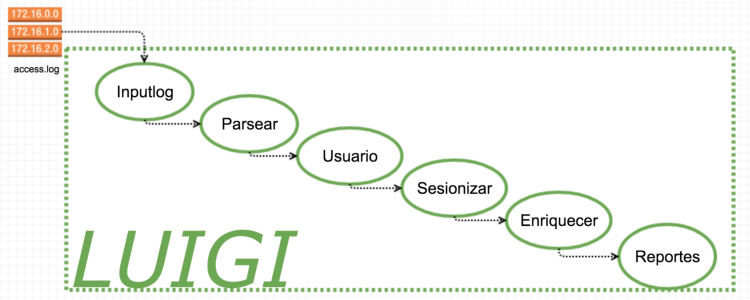
\includegraphics{entregable-analisis_clickstream_files/figure-latex/unnamed-chunk-1-1} \end{center}

\section{2. Instalación}\label{instalacion}

Para la ejecución del pipeline es necesario instalar \texttt{Python},
\texttt{R} y bibliotecas de \texttt{Python} usando \texttt{apt-get}

\begin{verbatim}
# Instalar R

    sudo apt-get update
    sudo apt-get install r-base
    
# Instalar dependencias de R

En la línea de comando para verificar la correcta instalación teclaer R

Entraras a la línea de comandos de R, teclear:

  install.packages("shiny")
  install.packages("dplyr")
  install.packages("ggplot2")
  
Una vez instalado las librerias, salir de R
  
  quit()

# Instalar Python

Volveras a la línea de comandos, teclear:

sudo apt-get install build-essential checkinstall
sudo apt-get install libreadline-gplv2-dev libncursesw5-dev \
libssl-dev libsqlite3-dev tk-dev libgdbm-dev libc6-dev libbz2-dev

sudo apt-get install python2.7

# Instalar dependencias de Python

  sudo pip install luigi
  sudo apt-get install python-matplotlib
\end{verbatim}

\subsubsection{3 Breve guía de uso}\label{breve-guia-de-uso}

Una vez instalado lo anterior, se necesitan 3 cosas para ejecutar el
pipeline correctamente, la función \emph{analisis-log-itam.py}, el
archivo \emph{access.log} y la carpeta de \emph{functions} la cuál trae
funciones externas. Lo necesario deberá estar en una ruta especificada
por el usuario.

En la línea de comandos ir hasta la ruta donde se tiene lo anterior

\begin{verbatim}
Ejemplo:
  cd User/miruta/misarchivos
  
\end{verbatim}

Para ejecutar el pipeline y visualizar el proceso es necesario abrir
otra línea de comandos y el navegador

\begin{verbatim}
Dentro de la línea de comandos teclear:

  luigid

Dentro del navegador, abrir el puerto y poner la siguiente dirección:

  http://localhost:8082/static/visualiser/index.html#
\end{verbatim}

Posteriormente en la línea de comandos (diferente a donde se tecleo
\emph{luigid}), ejecutar la función.

\begin{verbatim}
python analisis-log-itam.py Enriquecer --input-file access.log --output-file\
usuario.pd  --output-df sesionizar.pd --output-df1 enriquecer --output-df2\
reporte.pd
\end{verbatim}

La salida que se obtendrá será la siguiente

\begin{verbatim}
===== Luigi Execution Summary =====

Scheduled 5 tasks of which:
* 1 present dependencies were encountered:
    - 1 Inputlog(filename=access.log)
    
* 4 ran successfully:

    - 1 Sesionizar(input_file=access.log, output_file=usuario.pd,
    output_df=sesionizar.pd, output_df1=enriquecer)
    - 1 Parsear(input_file=access.log, output_file=usuario.pd)
    
    - 1 Enriquecer(input_file=access.log, output_file=usuario.pd,
    output_df=sesionizar.pd, output_df1=enriquecer, output_df2=reporte.pd)
    
    - 1 Usuario(input_file=access.log, output_file=usuario.pd, output_df=sesionizar.pd)

This progress looks :) because there were no failed tasks or
missing external dependencies

===== Luigi Execution Summary =====
\end{verbatim}

Una vez ejecutado, dentro de la ruta se crearan 5 archivos que son los
outputs descritos con anterioridad \emph{reporte.pd},
\emph{sesionizar.pd}, \emph{usuario.pd} y \emph{enriquecer.csv}

Dentro de la página que abriste con anterioridad se tendrá la siguiente
vista:

\begin{center}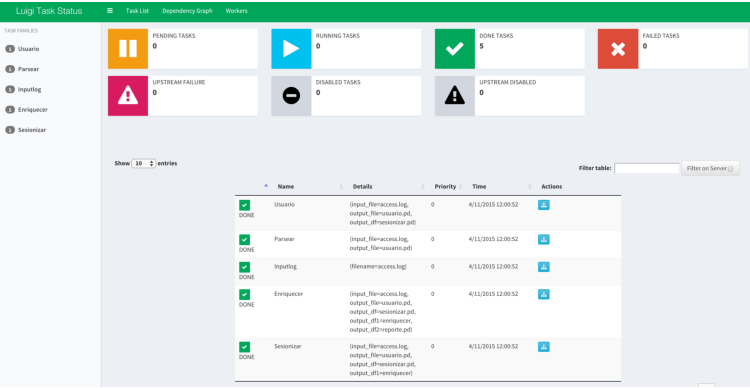
\includegraphics{entregable-analisis_clickstream_files/figure-latex/unnamed-chunk-2-1} \end{center}

\begin{center}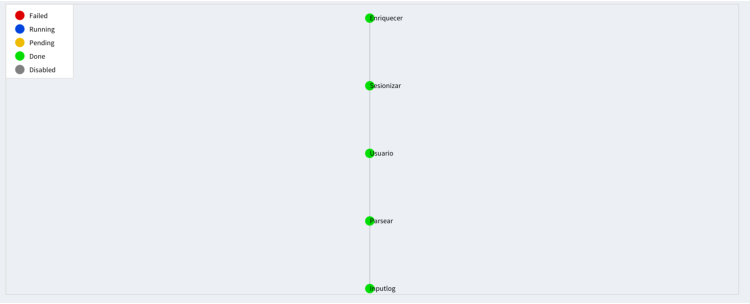
\includegraphics{entregable-analisis_clickstream_files/figure-latex/unnamed-chunk-3-1} \end{center}

\subsection{3.1 Ejecución Dashboard}\label{ejecucion-dashboard}

Para poder ejecutar el dashboard es necesario que en la ruta
especificada por el usuario (la cual debe ser la misma donde se
obtuvieron los outputs y el archivo enriquecer.csv), es necesario tener
la carpeta \emph{/R} la cual a su vez tiene dos archivos \emph{server.R}
y \emph{ui.R}

Nuevamente en la línea de comandos, ejecutar:

\begin{verbatim}
R -e "shiny::runApp('~/User/.../R/shinyapp’)"
\end{verbatim}

Al ejecutarse, se tendrá la siguiente salida:

\begin{verbatim}
> shiny::runApp('~/Desktop/conacyt/R/shinyapp')
Loading required package: shiny
This version of Shiny is designed to work with htmlwidgets >= 0.4. 
Please upgrade your version of htmlwidgets.


Listening on http://127.0.0.1:5127
\end{verbatim}

El puerto donde se ejecuta el dashboard será el hostname que se muestra,
el cual se tendrá que copiar y pegar en el navegador para poder observar
el dashboard.

Si todo es correcto, se mostrará lo siguiente:

\begin{center}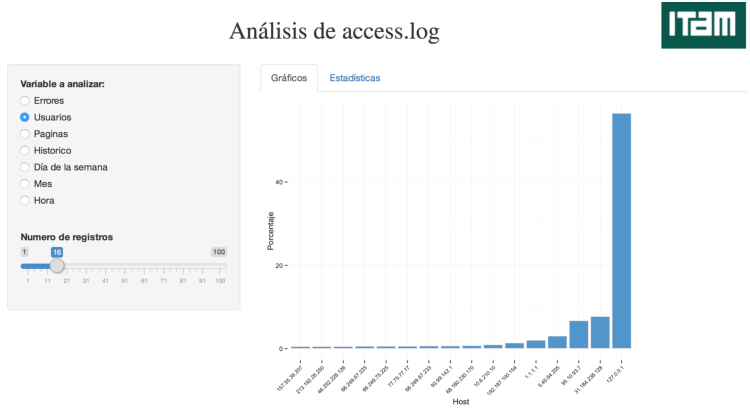
\includegraphics{entregable-analisis_clickstream_files/figure-latex/unnamed-chunk-4-1} \end{center}

\begin{center}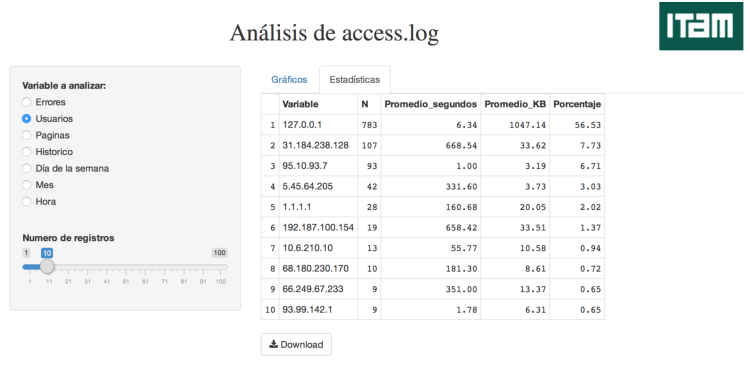
\includegraphics{entregable-analisis_clickstream_files/figure-latex/unnamed-chunk-5-1} \end{center}

En la parte del dashboard, además de poder visualizar las estadísticas
de las variables más importantes, se podrá descargar en formato
\emph{csv} la consulta que le interese al usuario y si esta no le
satisface, podrá descargar los insumos completos.

\subsubsection{Referencias}\label{referencias}

\begin{quote}
Andersen, J., Larsen, R. S., Giversen, A., Pedersen, T. B., Jensen, A.
H. y Skyt, J. (2000). Analyzing clickstreams using subsessions
\end{quote}

\begin{quote}
Banerjee, A., y Ghosh, J. (2002). Characterizing visitors to a web site
across multiple sessions. En Proceedings of NGDM'02: National Sci- ence
Foundation Workshop on Next Generation Data Mining. Mar- riott Inner
Harbor, Baltimore, MD, Estados Unidos.
\end{quote}

\begin{quote}
Lagus, K. (2000). Text mining with the websom. Tesis doctoral, Helsinki
University of Technology, Neural Networks Research Centre, Espoo,
Finlandia.
\end{quote}

\url{http://httpd.apache.org/}

\url{https://wiki.duraspace.org/}

\url{http://www.edu4java.com/}

\url{http://www.programcreek.com/2013/04/what-is-servlet-container/}

\end{document}
